% !TEX root = ../../main.tex

% ----------------------------------
% labels: \label{mil4:[type]:[name]}
% ----------------------------------
% FUTURE TENSE


Quantum fluctuations from the early universe generates inhomogeneity in the form of (energy) density enhancements and deficits. The rapid expansion during inflation stretches these quantum fluctuations to cosmic scales. From this, local fluctuations in the gravitational potential are implied. The primordial plasma compresses in potential wells found in regions of high density. Analogously, the tightly coupled plasma rarefies in potential hills created in regions of low density. These mechanisms generate pressure waves propagating at the speed of sound, eventually imprinting a pattern of sound in the CMB temperature. Unless otherwise stated, compressions and decompressions in a fluid are seen from the point of view of the potential \emph{well}.

Where the fluid is compressed in a well and thus heated, there is a region \emph{nearby}\footnote{Near enough to be in causal contact with the aforementioned density enhancement.} where the fluid expands on a hill and cools down. It is convenient to decompose the fluctuations into plane wave-modes that evolve independently, as we did in~\cref{sec:mil3}. Now, if such a mode corresponds to a wavelength that is shorter than the particle horizon, \emph{and} the photons are tightly coupled to the baryons, the temperature fluctuation will oscillate in time as the fluid compresses and rarefies. At recombination, sound waves stop oscillating and are frozen in. The last scattering surface corresponds to a maximal length for these sound waves to have travelled; the sound horizon at decoupling, briefly mentioned in~\cref{sec:mil2}. There is then a mode ($k_1$) that had just enough time to compress once, necessarily with half a wavelength equal this distance. The mode ($k_2$) with this distance as its whole wavelength, will have completed one cycle of compression/decompression at decoupling. These modes (2\textpi~over comoving wavelength) are then $k_n=n\pi/s_*$, where $n\in \mathbb{N}$ by extension.

Now, the perturbations from~\cref{sec:mil3} can be combined with an estimate of the post-inflation dilated quantum fluctuations to form theoretical power spectra, in particular those of the photon temperature and non-relativistic matter today. We will in this section produce these observables using the simplest concordance model of inflation. 

\subsection{Theory}\label[sec]{mil4:sec:theo}
% ---------------------------------------
% labels: \label{mil2:theo:[type]:[name]}
% ---------------------------------------
% PRESENT/FUTURE TENSE

\begin{itemize}
    \item Thermal history
    \item Thomson scattering
    \item Recombination: Saha and Peebles
    \item Sound horizon
\end{itemize}

Following the Big Bang Nucleosynthesis (BBN), ordinary matter in the universe 

\colorbox{pink}{\dots \, \dots \, \dots \, \dots \, \dots \, \dots \, \dots }


\subsubsection{Optical depth and visibility}\label[sec]{mil2:theo:sec:optical_depth}
    Photons travelling through a medium may be absorbed. The intensity of light emitted from a distance $x$ is reduced by the factor $\eu^{-\tau(x)}$ where $\tau(x)$ is the optical depth of the medium. In cosmology, Thomson scattering ($\gamma + e^{-} \rightleftharpoons \gamma+ e^{-}$) is predominantly responsible for the absorption of photons universe. This, and the assumption that the universe is transparent today, gives us the ODE for $\tau(x)$,
    \begin{equation}\label{mil2:theo:eq:ode_tau_of_x}
        \dv{\tau}{x} = - \frac{cn_e \sigma\ped{T}\eu^{x}}{\Hp(x)},
    \end{equation}
    with $\tau(0)=0$, where $\sigma\ped{T}$ is the Thomson scattering cross-section and $n_e$ the electron density. A related quantity is the visibility function
    \begin{equation}\label{mil2:theo:eq:gt_of_x}
        \gti(x)= - \eu^{-\tau(x)} \dv{\tau}{x},
    \end{equation}
    a proper probability distribution obeying $\int_{-\infty}^{0}\diff x\, \gti(x) = 1$. This function will have a peak at the point in time where the photons's mean free path increased tremendously, i.e. at the last scattering surface, which happened immediately after the number of free electrons dropped dramatically, i.e. recombination. In mathematical terms, $\gti(x\ped{lss}) = \max{\gti(x)}$.
    % \begin{equation}\label{mil2:theo:eq:def_of_lss}
    %     \gti(x\ped{lss}) = \max{\gti(x)}.
    % \end{equation}
    \colorbox{green}{more here!}

\subsubsection{Hydrogen recombination}\label[sec]{mil2:theo:sec:recombination}
    Before we can compute the optical depth, we need to know the electron number density, $n_e$, at all times. We define the free electron fraction $X_e\equiv n_e/n\ped{b}$ where $n\ped{b}$ is the total baryon number density. Before recombination, that is for $x<x_*$, all hydrogen is completely ionised, meaning that $X_e(x\!<\!x_*)\simeq 1$. We will let the time of recombination, $x_*$, be the solution to $X_e(x\!=\!x_*) = 0.1$.

    \colorbox{pink}{\dots \, \dots \, \dots \, \dots \, \dots \, \dots \, \dots }

    Consider the interaction that keeps electrons ($e^{-}$) and protons ($p$) in equilibrium with photons ($\gamma$),
    \begin{equation}\label{mil2:theo:eq:relevant_interaction}
        e^{-} + p \rightleftharpoons \element{H}+\gamma.
    \end{equation}
    Letting $n_s$ ($n_s^{(0)}$) denote the number density of a species/element $s$ (in equilibrium), the corresponding equilibrium equation is 
    \begin{align}\label{mil2:theo:eq:org_Saha}
        \frac{n_e n_p}{n\ped{\element{H}}}  = \frac{n_e^{(0)} n_p^{(0)}}{n\ped{\element{H}}^{(0)}},
    \end{align}
    the \textit{Saha equation}. Likewise letting $m_s$ refer to the mass of $s$, we can take the number density of neutral hydrogen to be
    \begin{equation}
        n\ped{H}= \left(1-Y_P\right) n\ped{b} \simeq \left(1-Y_P\right) \frac{\Omega\ped{b0}\rho\ped{cr0}}{m\ped{H}\eu^{3x}}\,;\quad \rho\ped{cr0} = \frac{3H_0^2}{8\pi G},
    \end{equation}
    where $Y_P$ denotes the primordial helium mass fraction. We neglect helium s.t. $Y_P = 0$ and assume that all baryons are protons. Further, recognising the neutrality of the universe ensures $n_p=n_e$. Now, $n\ped{b}=n_p + n\ped{\element{H}}$ and
    \begin{equation}
        X_e = \frac{n_e}{n_e + n\ped{\element{H}}} = \frac{n_p}{n_p + n\ped{\element{H}}}.
    \end{equation}
    Revisiting the reaction in \cref{mil2:theo:eq:relevant_interaction}

    \colorbox{pink}{\dots \, \dots \, \dots \, \dots \, \dots \, \dots \, \dots }
    
    Let $\varUpsilon\equiv \epsilon_0/(k\ped{B} T\ped{b} )$ for notational ease. Multiplying \cref{mil2:theo:eq:org_Saha} by $n\ped{b}^{-1}$ and inserting expressions for $n_s^{(0)}$, we obtain the more useful form of the Saha equation
    \begin{equation}\label{mil2:theo:eq:Saha}
        \frac{X_e^2}{1-X_e}= \frac{1}{n\ped{b}}\left(\frac{m_e k\ped{B} T\ped{b}}{2\pi \hbar^2} \right)^{\sfrac{3}{2}} \eu^{-\epskT}\,; \quad   0 < X_e \leq 1 \wedge X_e\sim 1.
    \end{equation}
    The constraints on $X_e$ are that it is a positive number that cannot exceed 1 and the observation that it has to be close to 1. The latter constraint is due to the equilibrium assumption from which the Saha equation is derived: as $X_e$ falls the reaction rate for \cref{mil2:theo:eq:relevant_interaction} falls and equilibrium is not guaranteed. To proceed, we need to solve the Boltzmann equation. More precisely, James Peebles needed to solve the Boltzmann equation, whereas we will study the product; a first-order ODE the \textit{Peebles equation}. Said equation reads
    \begin{equation}\label{mil2:theo:eq:Peebles}
        \dv{X_e}{x} = \frac{C_r(T\ped{b})}{\Hp(x)\eu^{-x}} \left[ \beta(T\ped{b}) \left(1-X_e\right) - n\ped{\element{H}} \alpha^{(2)}(T\ped{b})X_e^2 \right],
    \end{equation}
    % .... the change in $X_e$ with respect to $x$ goes as the reduction factor $C_r$, times the collisional ionisation rate from the ground state
    where the necessary mathematical expressions are found in \cref{mil2:theo:eq:Peebles_add}.

    Let us break the equation down to physical quantities and processes. 
    \begin{itemize}
        \item The net effect of a ground-state recombination is zero.
        \item \dots
        \item There are to pathways from the first excited state $n=2$ to the ground state $n=1$: \begin{itemize}
            \item $2p\to 1s$: decay through the emission of a Lyman-\textalpha~photon (rate given by $\Lambda_\alpha$ in \cref{mil2:theo:eq:Peebles_Lambda_alpha}) something about cosmological redshift
            \item $2s\to 1s$: 2-photon decay (rate given by $\Lambda_{2s\to 1s}$ in \cref{mil2:theo:eq:Peebles_Lambda_2s1s})
        \end{itemize} 
        \item \dots
    \end{itemize}
    The reduction (or correction) factor $C_r$ is the ratio between the net decay rate and the combined decay and ionisation rate () from the first excited level ($n=2$) (see \cref{mil2:theo:eq:Peebles_Cr}).
    \citep{DodelsonBook,ChungPei1995,Peebles1968}

    \colorbox{pink}{\dots \, \dots \, \dots \, \dots \, \dots \, \dots \, \dots }

    \begin{subequations}\label{mil2:theo:eq:Peebles_add}
        \begin{align}
            C_r(T\ped{b}) &= \frac{\Lambda_{2s\to 1s}+ \Lambda_{\alpha}}{\Lambda_{2s\to 1s} + \Lambda_\alpha + \beta^{(2)}(T\ped{b})} \label{mil2:theo:eq:Peebles_Cr} \\
            \Lambda_{2s\to 1s} &=8.227\unit{s}^{-1} \label{mil2:theo:eq:Peebles_Lambda_2s1s}  \\
            \Lambda_\alpha &= \frac{\Hp\eu^{-x}}{(8\pi)^2 n_{1s}}\left( \frac{3\epsilon_0}{\hbar c}\right)^3 \label{mil2:theo:eq:Peebles_Lambda_alpha}  \\
            n_{1s} &= (1-X_e)n\ped{H}\label{mil2:theo:eq:Peebles_n1s}\\
            \beta^{(2)}(T\ped{b}) &= \beta(T\ped{b})\eu^{\sfrac{3}{4}\epskT} \label{mil2:theo:eq:Peebles_beta2} \\
            \beta (T\ped{b}) &= \alpha^{(2)}(T\ped{b}) \left(\frac{m_e k\ped{B} T\ped{b}}{2\pi \hbar^2} \right)^{\sfrac{3}{2}} \eu^{-\epskT} \label{mil2:theo:eq:Peebles_beta}  \\
            \alpha^{(2)}(T\ped{b}) &= \frac{8}{\sqrt{3\pi}} c\sigma\ped{T} \sqrt{\epskT} \phi_2(T\ped{b}) \label{mil2:theo:eq:Peebles_alpha2} \\
            \phi_2(T\ped{b}) &= 0.448\ln{\epskT} \label{mil2:theo:eq:Peebles_phi2}
        \end{align}
    \end{subequations}


\subsubsection{Sound horizon}\label[sec]{mil2:theo:eq:sound_horizon}
    The distance that a sound wave could propagate in the primordial plasma before photons decoupled is called ``the sound horizon at decoupling'', a quantity whose significance will become prominent in sections to come. We define the sound speed of a photon-baryon plasma as
    \begin{equation}
        c_s \equiv c\sqrt{\frac{1}{3(1+R(x))}}.
    \end{equation}
    where the baryon-to-photon energy density is defined as
    \begin{equation}
        R(x) \equiv \frac{3\Omega\ped{b0}}{4\Omega\gped{\textgamma 0}}\eu^x.
    \end{equation}
    The comoving distance traveled by a sound wave -- the sound horizon -- at time $x$ as the solution $r_s(x)$ to the ODE
    \begin{equation}
        \dv{r_s}{x} = \frac{c_s}{\Hp(x)}\, ; \quad r_s(x\ped{init}) = \frac{c_s(x\ped{init})}{\Hp(x\ped{init}) }.
    \end{equation}
    Evaluating $r_s(x=x\ped{dec})$ gives the sound horizon at decoupling.


\subsection{Implementation details}\label[sec]{mil4:sec:imp}
% !TEX root = ../../main.tex

% --------------------------------------
% labels: \label{mil4:imp:[type]:[name]}
% --------------------------------------
% PAST TENSE



% \begin{equation}\label{mil4:imp:eq:trapezoidal_uniform}
%     \int_{a}^{b} \dx{z} f(z) \approx \Delta z \left( \sum_{j=1}^{N-1}f(z_j) + \frac{f(z_0) + f(z_{N})}{2} \right)\,; \quad \Delta z= \frac{b-a}{N}
% \end{equation}

We wrote a \verb|C++| code that uses the class objects from the previous sections and three additional parameters; primordial amplitude $\mathcal{A}\ped{S}$, spectral index $n\ped{S}$ and pivot scale $k\ped{p}$. We used the following fiducial values:
\begin{equation}
\begin{split}
    \mathcal{A}\ped{S}  &=  2.1\cross 10^{-9}   \\
    n\ped{S}            &=  0.965               \\
    k\ped{p}            &=  0.05\unit{Mpc^{-1}}
\end{split}
\end{equation}


There were three main computations to this problem: the work of finding $j_\ell(z)$, where $z= k(\eta_0-\eta(x))$, and $\Theta_\ell(0,k)$ for a set of $\ell$s, then computing (and interpolating) $C(\ell)$.
% for $\ell=2,3, \dots,\ell\ped{MAX}$, where $\ell\ped{MAX}=2000$ is where we stop the line-of-sight integration from \textcolor{blue}{(ref to sec.!)}. 
We do not solve any differential equations, but rather use the very powerful trapezoidal rule to evaluate our integrals. For a fixed step size $\Delta z$, this rule takes the simple form
\begin{equation}\label{mil4:imp:eq:trapezoidal_uniform}
    \int_{z_0}^{z_N} \dx{z} f(z) \approx \Delta z \left( \sum_{j=1}^{N-1}f(z_j) + \frac{f(z_0) + f(z_{N})}{2} \right)\,; \quad N= \frac{z_N-z_0}{\Delta z}.
\end{equation}


In preparation of the necessary computations, we chose a set of $\ell$s, call it $L$, for which to perform the line-of-sight integration. We let $L\subset \mathcal{L}\equiv \{\,2,\,3,\, \dots,\,  \ell\ped{MAX}\,\}$ be a clever choice of a number of integers\footnote{63, to be exact.} $\ell\in \mathcal{L}$. The resolution in the subdomain $L$ needs to be such that oscillatory information is not lost in going from $C(\ell\in L)\to C(\ell\in\mathcal{L})$. We let $\ell\ped{MAX}=2000 \in L$ be the highest multipole we consider. 

% GSL: "http://www.gnu.org/software/gsl/"
% BESSEL FUNCTIONS
To generate the spherical Bessel functions, we utilised the functionalities of GSL. We loop through $\ell \in L$ and, for each iteration, collected the $j_\ell(z)$'s from GSL for $z=0,\,\Delta z,\, 2\Delta z,\, \dots,\, k\ped{max}\eta_0$, where $\Delta z = 2\pi/n\ped{samp}$. To properly sample the oscillations, we used $n\ped{samp}=20$. 

% LOS INTEGRATION
For the computation of $\Theta_\ell(0,k)$, we designed a grid of $\ell$, $k$ and $x$-values. Naturally, we considered $\ell \in L$. The resolution for $k\in [k\ped{min},\,k\ped{max}]$ will be addressed shortly. The integration in~\cref{mil4:theo:eq:los_integration} was started from $x=-8.3$ with step size $\Delta x= 2\pi/n\ped{samp}$ in~\cref{mil4:imp:eq:trapezoidal_uniform}. This time we used $n\ped{samp}=500$. 

% C(\ell) COMPUTATION
We solved~\cref{mil4:theo:eq:C_of_ell_final} for $C(\ell\in L)$ using the trapezoidal rule in~\cref{mil4:imp:eq:trapezoidal_uniform} with $z\to\ln{k}$. That is, we solved
\begin{equation}
    C(\ell) = 4\pi \int_{\ln{k\ped{min}}}^{\ln{k\ped{max}}} \dx{\ln{k}} \abs{\Theta_\ell(0,k)}^2 \Delta_\mathcal{R}^2(k)
\end{equation}
with a fixed step size $\Delta\!\ln{k}$. \textcolor{blue}{EXPLAIN k-ARRAY}

\subsection{Results}\label[sec]{mil4:sec:res}
% !TEX root = ../../main.tex

% --------------------------------------
% labels: \label{mil4:res:[type]:[name]}
% --------------------------------------
% PAST TENSE


As functions of wavenumber $k$, we plot the transfer function for a set of angular wavenumbers $\ell \in \{\, 6,\, 100,\, 200,\, 500,\, 1000 \,\}$ in~\cref{mil4:res:fig:transfer}. For the largest values of $k$, we also plot the interesting part of the integrand in the expression for the CMB power spectrum. 
\begin{figure}[!ht]
    \centering
    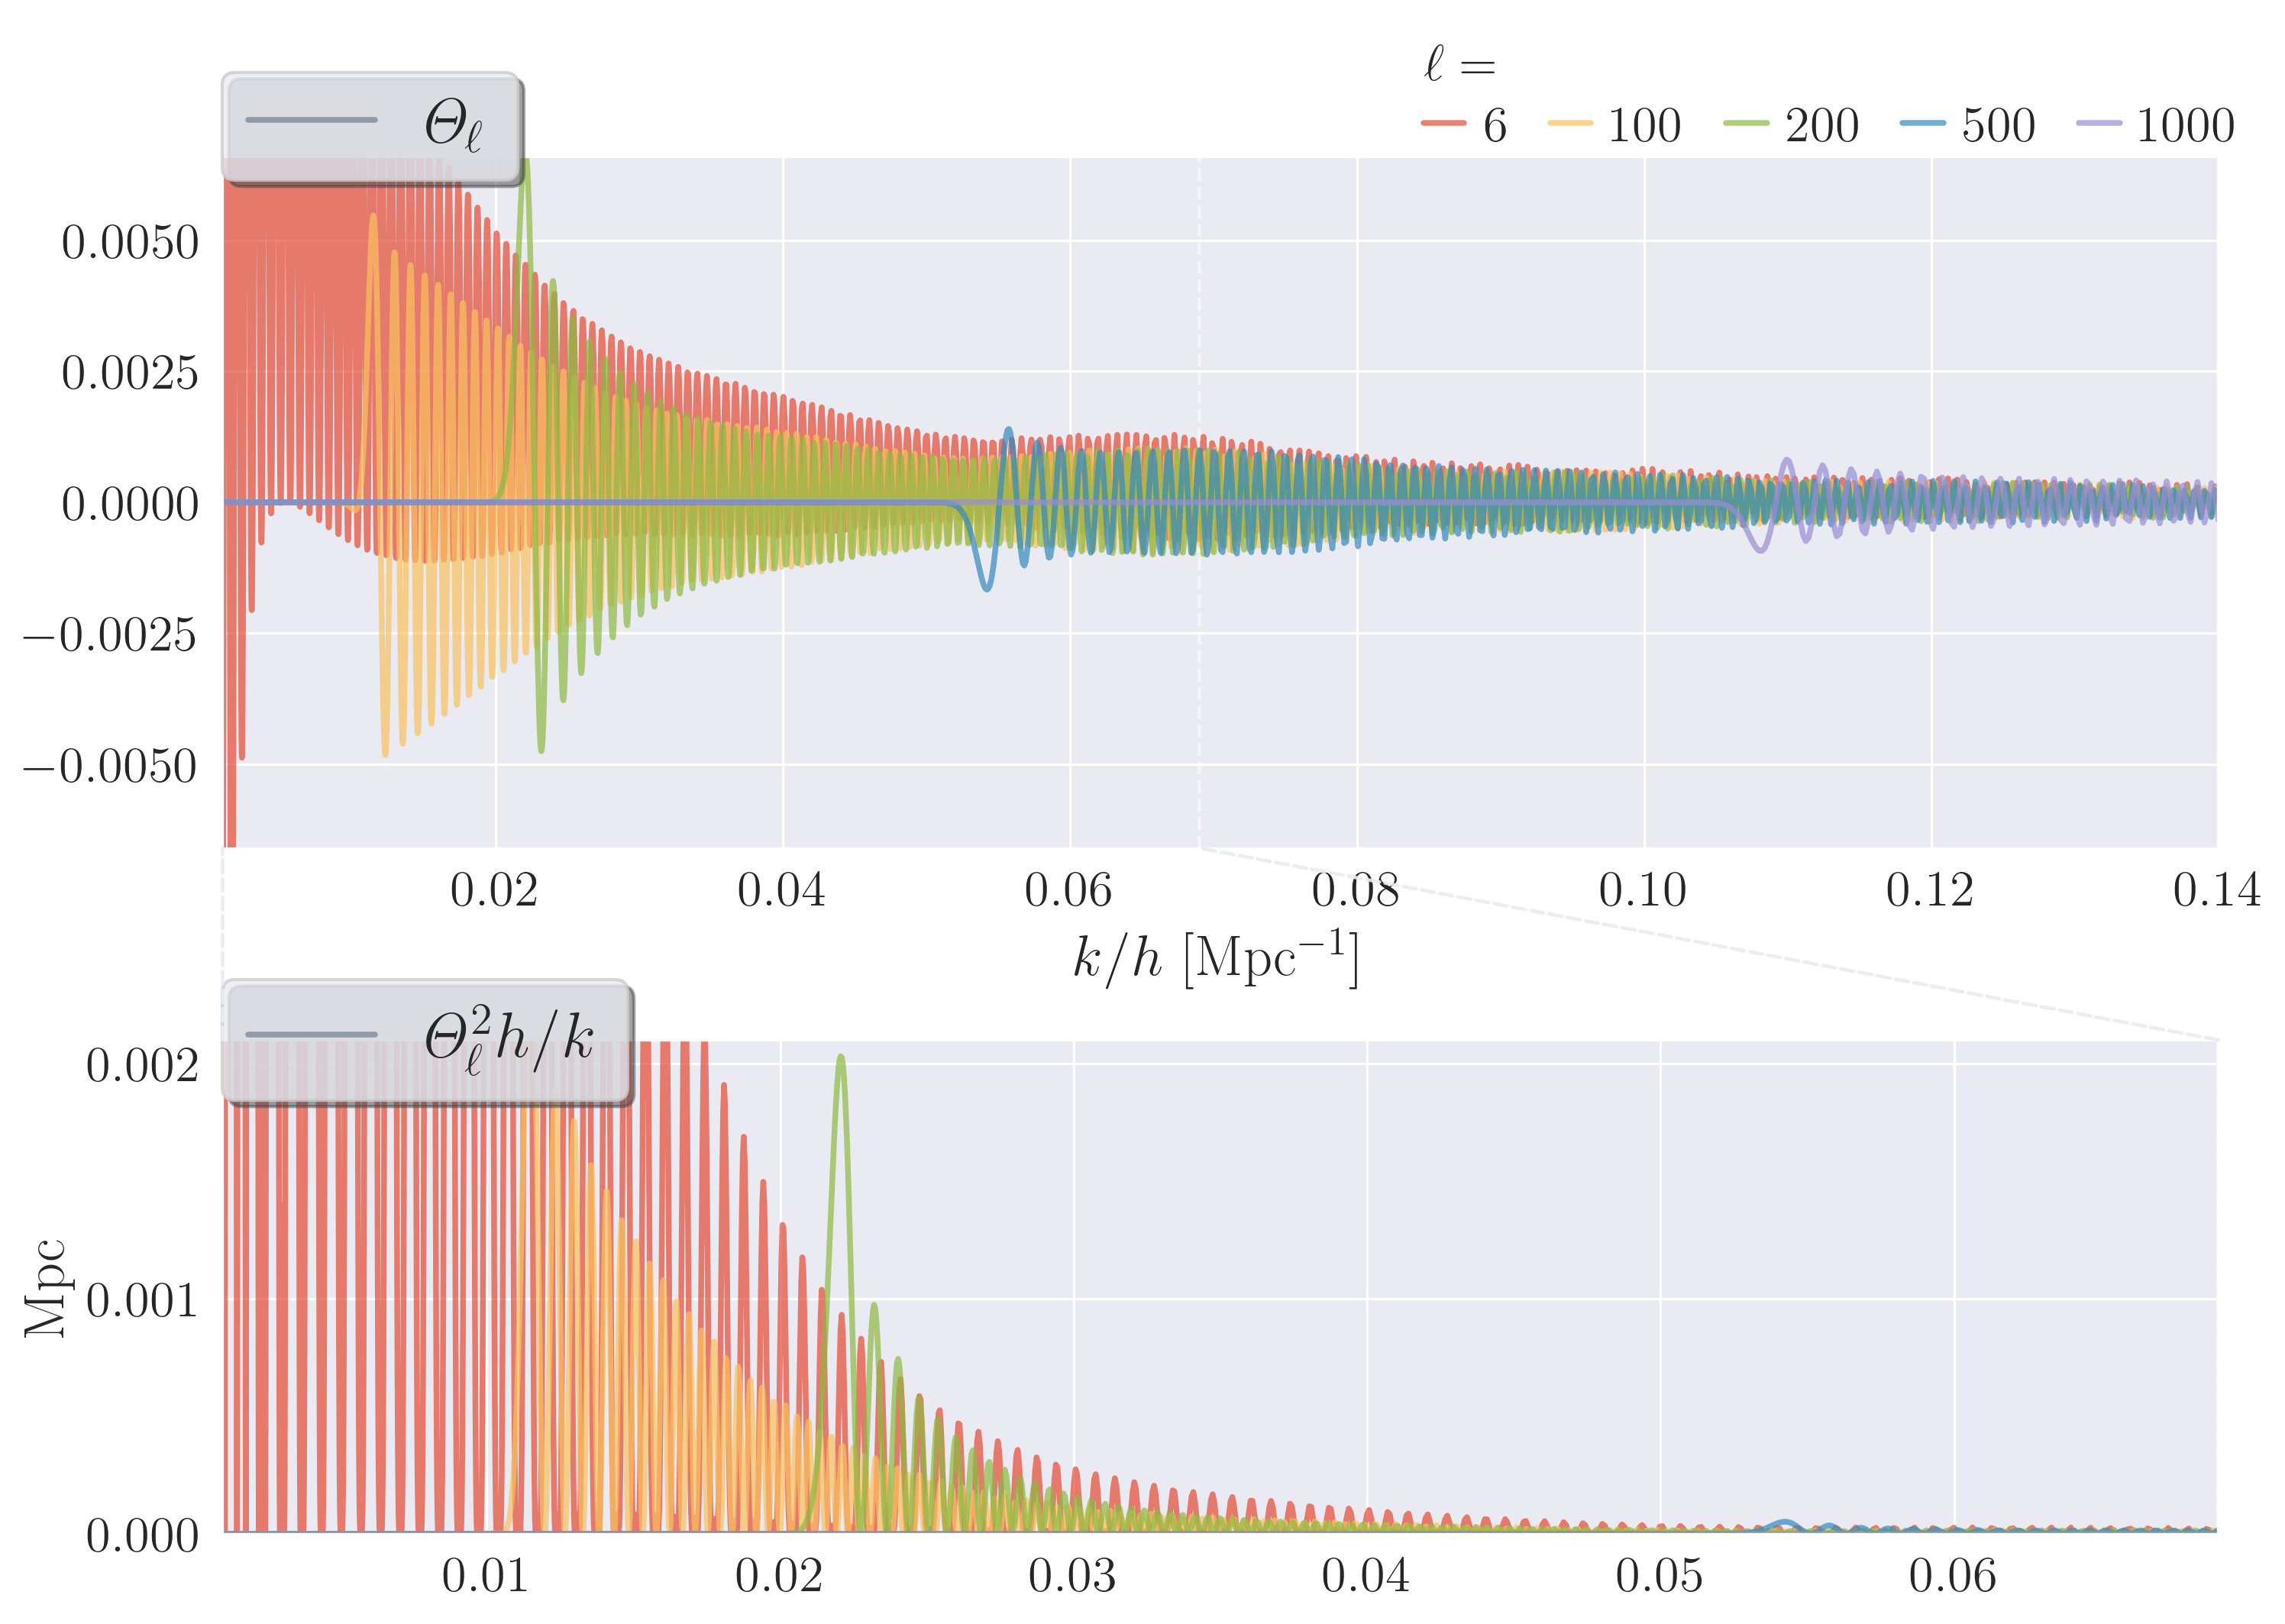
\includegraphics[width=\linewidth]{milestone4/Theta_ell.png} 
    \caption{The photon transfer functions $\Theta_\ell(x_0, k)$ as functions of wavenumber $k$ for a set of angular wavenumbers $\ell$. Upper panel: Plainly $\Theta_\ell(0, k)$. Lower panel: Squared and scaled $\frac{\Theta^2_\ell(0,k)}{k}$.} 
\label[fig]{mil4:res:fig:transfer}
\end{figure}

The CMB power spectrum is presented in~\cref{mil4:res:fig:CMB_power}. Note that we used the scaled quantity $\mathcal{D}(\ell)$. The different contributions to the CMB anisotropy were overplotted, as well as the cosmic variance from~\cref{mil4:theo:eq:cosmic_variance}. We included observational data from~\citet{Planckdata} for low $\ell$. Observational data become less relevant for $\ell \gtrsim 200$ as effects of e.g.\ neutrinos are non-negligible at these scales.
\begin{figure}[!ht]
    \centering
    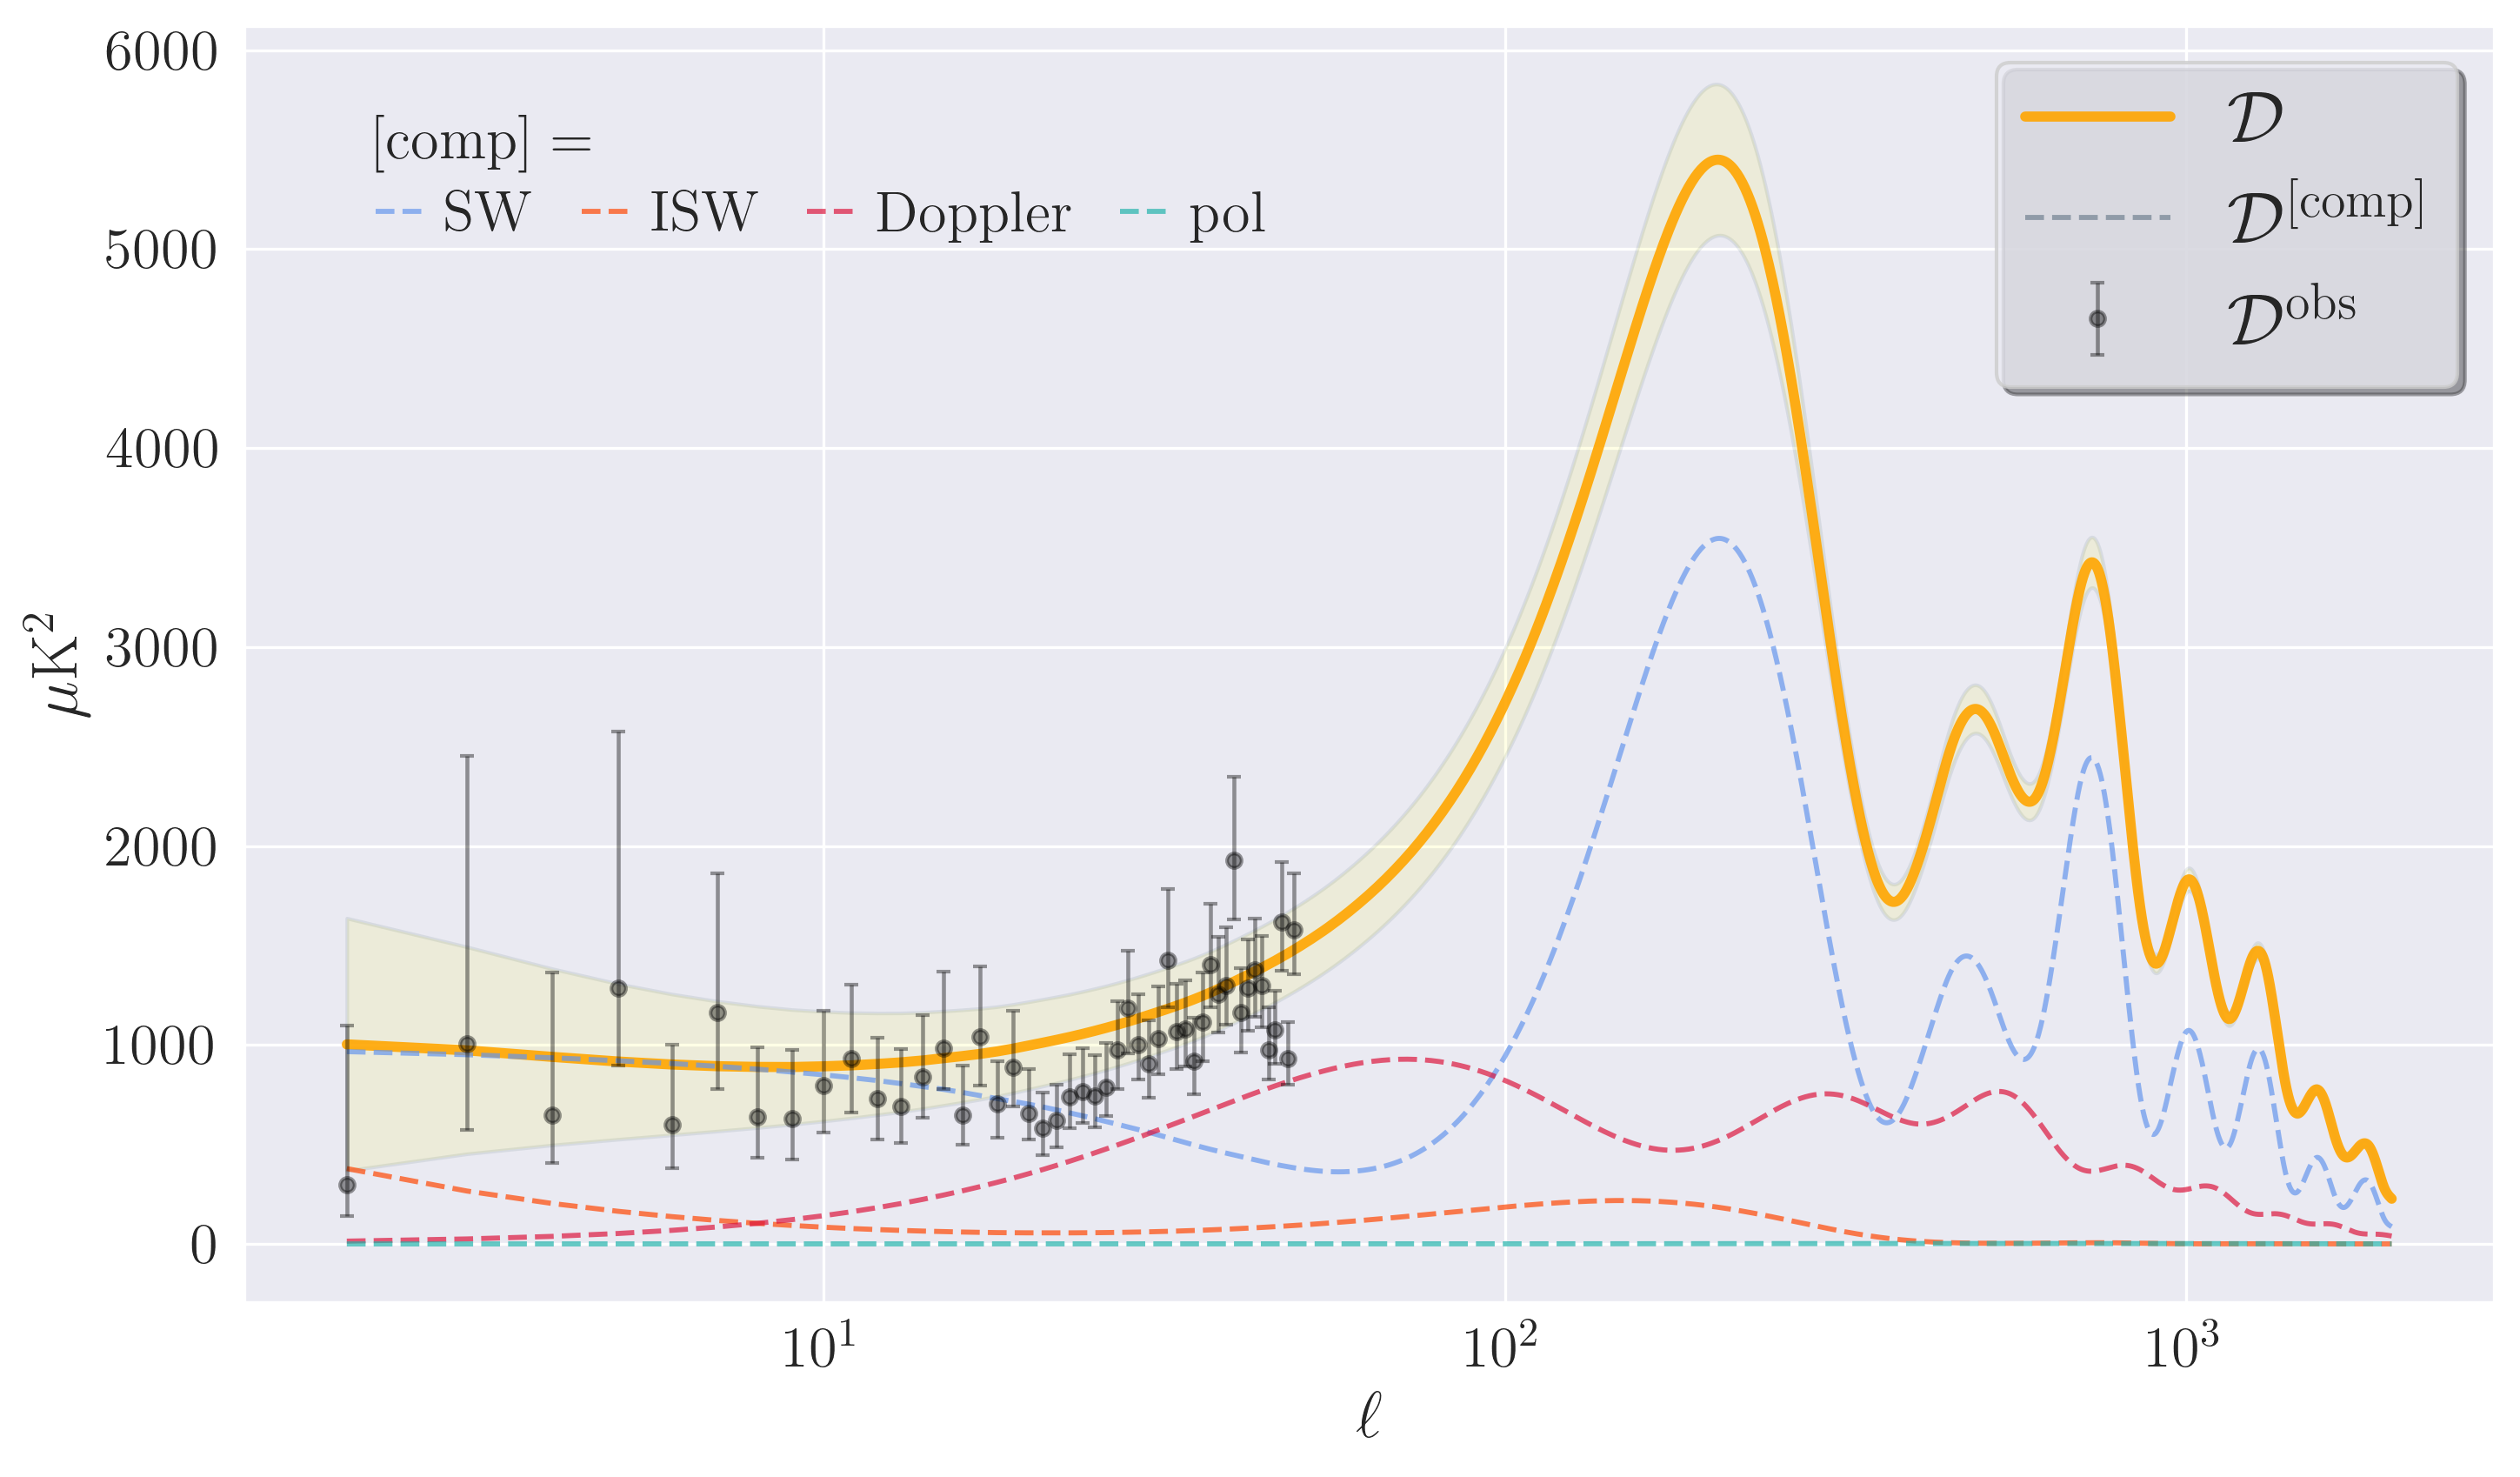
\includegraphics[width=\linewidth]{milestone4/CMB_power_spectrum.png} 
    \caption{The scaled CMB power spectrum $\mathcal{D}(\ell)$ as function of multipole moment $\ell$. The shaded region represents the fundamental cosmic variance. Upper axis demonstrates corresponding angular scale $\sim 180^\circ /\ell$.} 
\label[fig]{mil4:res:fig:CMB_power}
\end{figure}
The contributions to the CMB spectrum are calculated as follows, were $\mathrm{[comp]}\in \{\,\mathrm{SW},\,\mathrm{ISW},\,\mathrm{Doppler},\,\mathrm{pol} \,\}$ are the terms in the source function (\cref{mil4:theo:eq:source_function_four_terms}) given by~\cref{mil4:theo:eq:source_terms}:
\begin{equation}
\begin{split}
    &\mathcal{D}(\ell)^\mathrm{[comp]} = \frac{\ell (\ell +1 ) \TCMB^2}{2\pi} C(\ell)^\mathrm{[comp]}\,; \\
    &\quad C(\ell)^\mathrm{[comp]} =  4\pi \int_0^{\infty} \dx{k} \frac{\abs{\Theta_\ell^{\mathrm{[comp]}}(0,k)}^2}{k} \Delta_\mathcal{R}^2(k)\,; \\
    &\quad\quad \Theta_\ell^\mathrm{[comp]}(0,k) = \int_{-\infty}^0 \dx{x}(\mathrm{[comp]}) j_\ell(k\left[\eta_0 -\eta(x)\right] )
\end{split}
\end{equation}


In figure~\cref{mil4:res:fig:matter_power} is plotted the total matter power spectrum. Observational data from~\citet{wmap_act} and \textcolor{blue}{CITE} is shown in the same figure. Discrepancy is significantly larger for smaller scales.
\begin{figure}[!ht]
    \centering
    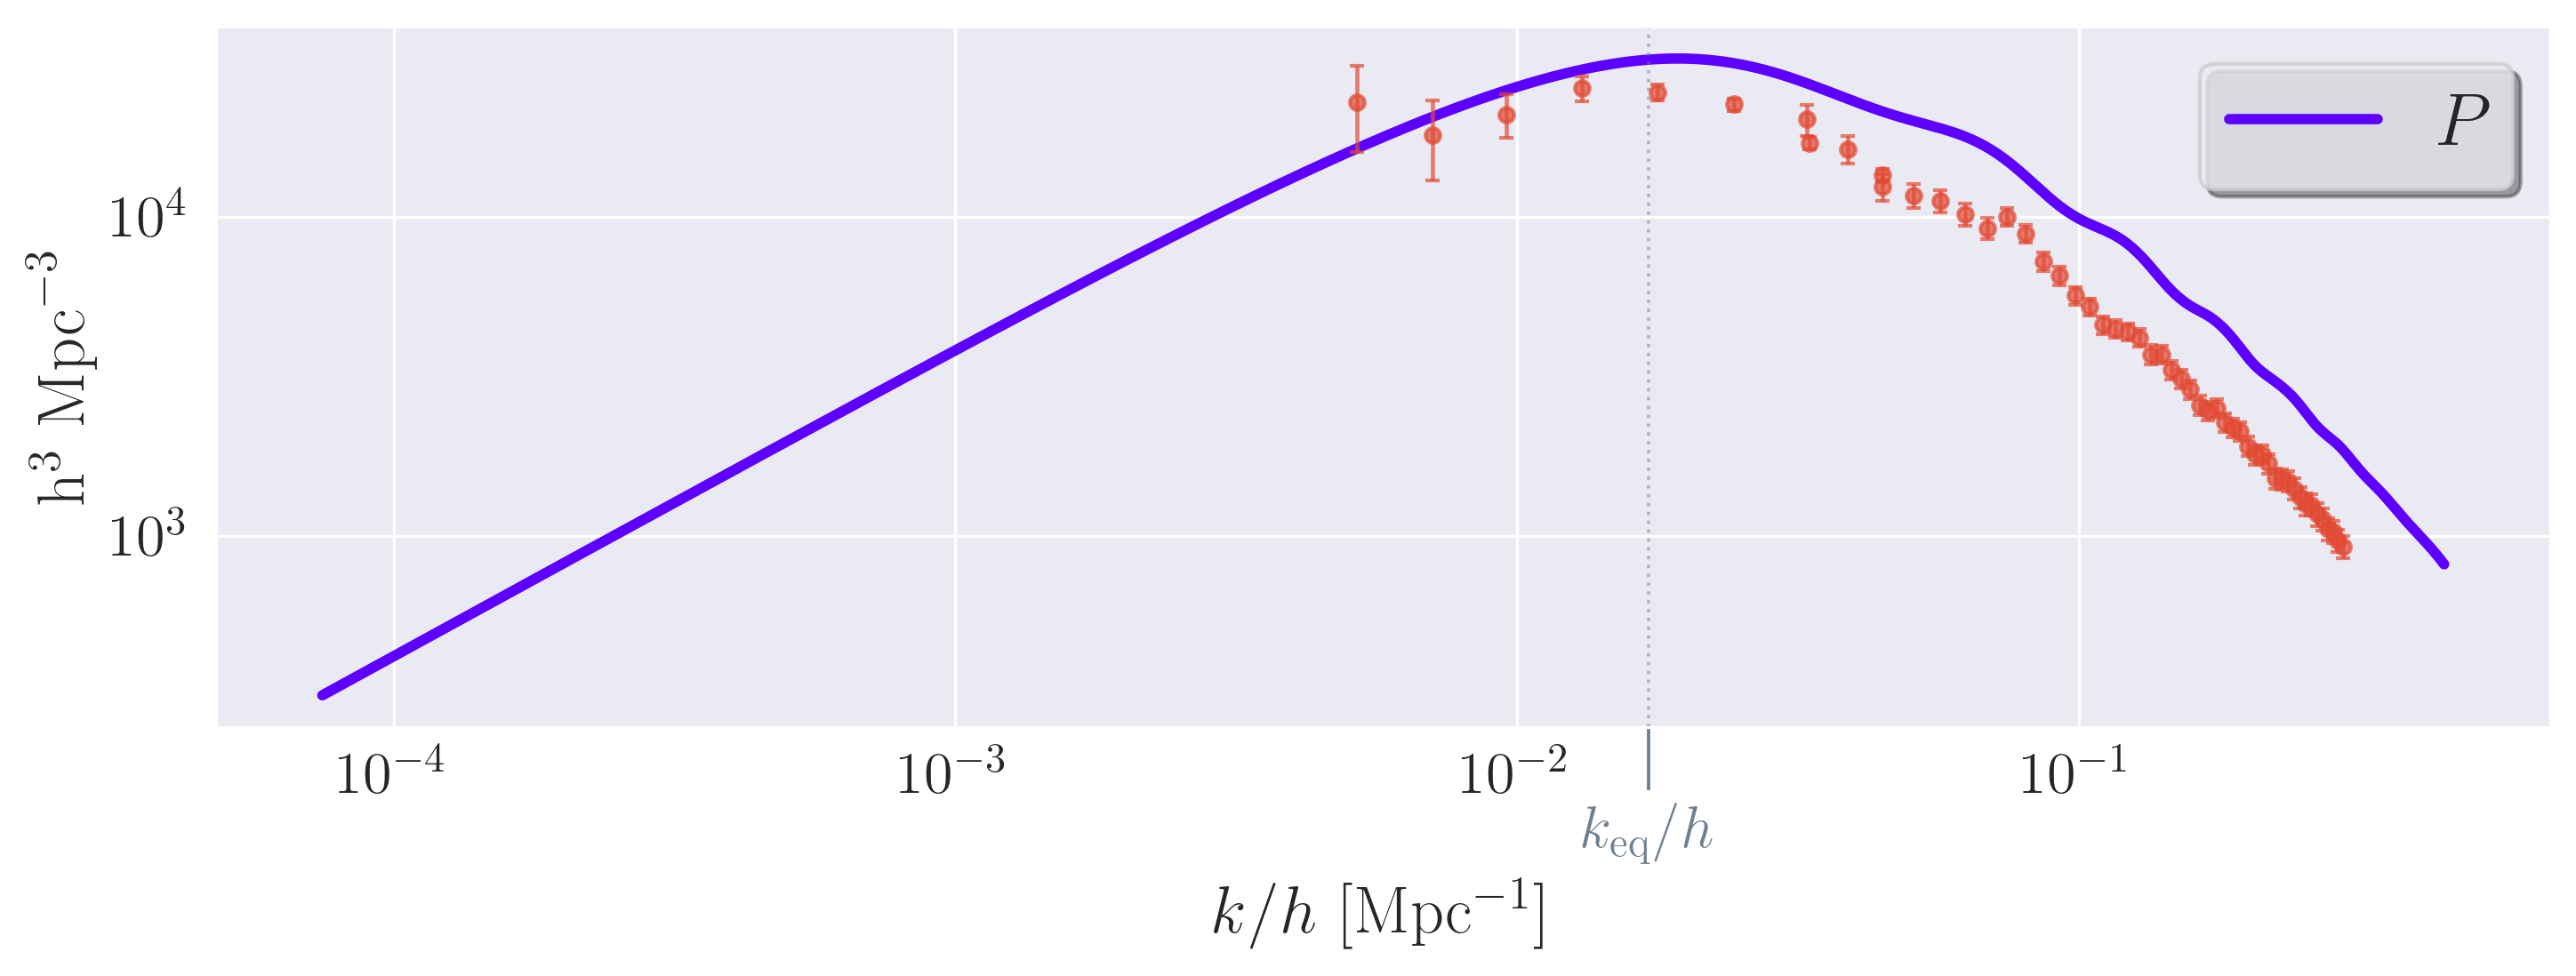
\includegraphics[width=\linewidth]{milestone4/matter_power_spectrum.png} 
    \caption{The total matter power spectrum (today) $P(0,k)$ as function of wavenumber $k$. Both axes are logarithmic. The equality scale $k\ped{eq}$ is demonstrated by a vertical dotted line.} 
\label[fig]{mil4:res:fig:matter_power}
\end{figure}

\subsection{Discussion}\label[sec]{mil4:sec:disc}
% !TEX root = ../../main.tex

% ---------------------------------------
% labels: \label{mil4:disc:[type]:[name]}
% ---------------------------------------
% PRESENT TENSE


The transfer functions in~\cref{mil4:res:fig:transfer} 



We turn to the main result of this project in~\cref{mil4:res:fig:CMB_power}. The Sachs-Wolfe and Doppler contributions to the CMB anisotropy are by far most significant in order to reproduce the observed spectrum. We spot the Sachs-Wolfe plateau for small $\ell$. The polarisation term is negligible in our model. 

The increasing significance of the integrated Sachs-Wolfe effect for smaller $\ell$ is visible in the plot. This is the late-time ISW large-scale effect kicking in as dark energy starts to dominate and thereby affect the gravitational potential in such a way that \textcolor{blue}{help}


We discuss below the different contributions to the CMB anisotropy in a systematical manner.

\dots

\dots 

\dots 

\dots

%  PEAKS
(ANGULAR PEAKS:) As we know, modes caught in states of extrema at the time of recombination make up the angular peaks---the peaks in the CMB power spectrum. We see that the mode that compressed once inside potential wells prior to recombination corresponds to an angular wavenumber $\ell\sim 200$, that is an angular size of $\sim 1^\circ$. 